\documentclass[]{article}
\usepackage{lmodern}
\usepackage{amssymb,amsmath}
\usepackage{ifxetex,ifluatex}
\usepackage{fixltx2e} % provides \textsubscript
\ifnum 0\ifxetex 1\fi\ifluatex 1\fi=0 % if pdftex
  \usepackage[T1]{fontenc}
  \usepackage[utf8]{inputenc}
\else % if luatex or xelatex
  \ifxetex
    \usepackage{mathspec}
  \else
    \usepackage{fontspec}
  \fi
  \defaultfontfeatures{Ligatures=TeX,Scale=MatchLowercase}
\fi
% use upquote if available, for straight quotes in verbatim environments
\IfFileExists{upquote.sty}{\usepackage{upquote}}{}
% use microtype if available
\IfFileExists{microtype.sty}{%
\usepackage{microtype}
\UseMicrotypeSet[protrusion]{basicmath} % disable protrusion for tt fonts
}{}
\usepackage[margin=1in]{geometry}
\usepackage{hyperref}
\hypersetup{unicode=true,
            pdfborder={0 0 0},
            breaklinks=true}
\urlstyle{same}  % don't use monospace font for urls
\usepackage{graphicx,grffile}
\makeatletter
\def\maxwidth{\ifdim\Gin@nat@width>\linewidth\linewidth\else\Gin@nat@width\fi}
\def\maxheight{\ifdim\Gin@nat@height>\textheight\textheight\else\Gin@nat@height\fi}
\makeatother
% Scale images if necessary, so that they will not overflow the page
% margins by default, and it is still possible to overwrite the defaults
% using explicit options in \includegraphics[width, height, ...]{}
\setkeys{Gin}{width=\maxwidth,height=\maxheight,keepaspectratio}
\IfFileExists{parskip.sty}{%
\usepackage{parskip}
}{% else
\setlength{\parindent}{0pt}
\setlength{\parskip}{6pt plus 2pt minus 1pt}
}
\setlength{\emergencystretch}{3em}  % prevent overfull lines
\providecommand{\tightlist}{%
  \setlength{\itemsep}{0pt}\setlength{\parskip}{0pt}}
\setcounter{secnumdepth}{0}
% Redefines (sub)paragraphs to behave more like sections
\ifx\paragraph\undefined\else
\let\oldparagraph\paragraph
\renewcommand{\paragraph}[1]{\oldparagraph{#1}\mbox{}}
\fi
\ifx\subparagraph\undefined\else
\let\oldsubparagraph\subparagraph
\renewcommand{\subparagraph}[1]{\oldsubparagraph{#1}\mbox{}}
\fi

%%% Use protect on footnotes to avoid problems with footnotes in titles
\let\rmarkdownfootnote\footnote%
\def\footnote{\protect\rmarkdownfootnote}

%%% Change title format to be more compact
\usepackage{titling}

% Create subtitle command for use in maketitle
\providecommand{\subtitle}[1]{
  \posttitle{
    \begin{center}\large#1\end{center}
    }
}

\setlength{\droptitle}{-2em}

  \title{}
    \pretitle{\vspace{\droptitle}}
  \posttitle{}
    \author{}
    \preauthor{}\postauthor{}
    \date{}
    \predate{}\postdate{}
  

\begin{document}

\doublespacing

\section{Introduction}
\label{sec3:Introduction}

The fundamental premise in the nature behind ORMFs, is to provide an
exposure-based treatment of OpRisk losses which caters to modeling
capital estimates for forward-looking aspects of ORM. This proves tricky
due to the need of specific knowledge about potential loss events as a
requirement, from the time the loss event occurs and the underlying
loss-generating mechanisms until the actual realised loss is realised.
By its very nature, this OpRisk type is characterised by a significant
lag between the moment the event is conceived to the point the event is
observed and accounted for.\medskip 

For example, in the case of rogue trading, there is a frequency exposure
associated with traders \emph{going rogue}, due to a probability of
rogue events happening between a specific group of traders, which is
then modeled for each rogue trading event and the impact (severity based
on the size of the position) of the loss when it is realised (at time of
detection). This timing paradox often results in questionable capital
estimates, especially for those near misses, pending and realised losses
that need to be captured in the model.

\section{Applicability of EBOR methodology for capturing forward-looking aspects of ORM}
\label{sec:Applicability of EBOR methodology for capturing forward-looking aspects of ORM}

By it's very nature, OpRisk has a significant lag usually characterised
by the time delay between the moment the OpRisk event is conceived up
until the moment the event is observed and accounted for, i.e., there is
a gap in time between the moment the risk is conceived and the realised
losses. A fundamental premise behind the tricky nature of ORMF, is to
provide an exposure-based treatment of OpRisk losses which caters for
modeling capital estimates of forward-looking aspects of ORM, due to the
lag in the loss data.\medskip

@einemann2018operational works unearth an invaluable contribution to the
literature, whereby the EBOR model is considered as an additional cell,
anagolously to the BL/ET matrix combinations in a classical LDA model,
therefore building hybrid frameworks when integrated with the LDA model
facilitating the migration of OpRisk types from a classical to an
exposure-based treatment through a quantitative framework
{[}@einemann2018operational{]}. Conceptually, the EBOR component can be
extended to include potential future events e.g., future litigations,
based on some underlying property, capturing forward looking aspects of
business environment and internal control factors (BEICF's)
thereof.\medskip

The fundamental premise behind the LDA is that each firm's OpRisk losses
are a reflection of it's underlying Oprisk exposure. OpRisk events
relating to a varying or constant degree of exposure need to take this
into account when modeling count or frequency of an event occuring. In
particular, the assumption behind the use of the Poisson distribution in
the model to estimate the frequency of losses, is that both the the
intensity (or rate) of occurrence and the opportunity (or exposure) for
counting can assume either of these two forms, for all available
observations {[}@dobson2008introduction{]}. In the former case the
varying degrees of exposure impact on the rate of events, whereas in the
latter case the exposure is constant hence not relevant to the
model.\medskip

When observed counts all have the same exposure, modeling the mean count
\(\mu\) as a function of explanatory variables \(x_{1},\ldots,x_{p}\) is
the same as modeling the rate \(R\). The actual measure of exposure we
need to use depends specifically on projecting the count of OpRisk
events (frequency of realised losses) as the target variable in the
model as opposed to the measure if the target variable were the severity
of the losses, whereby modeling for each rogue trading event the
severity based on size of loss position as severity exposure, and time
to detection or CapturedBy as severity risk factors.

\subsection{Definition of exposure}
\label{ssec:Definition of exposure}

Exposure is residual risk, or the risk that remains after risk
treatments have been applied. In the ORMF context, it is defined as:

\begin{definition}
The  \textbf{exposure} of risk type $i$, $d_{i}$ is the time interval, expressed in units of time, from the initial moment when the event happened, until the occurrence of a risk correction.
\end{definition}

As per definition \ref{ssec:Definition of exposure}, the lag represents
exposure; we need historical exposure for experience rating because we
need to be able to compare the loss experience of different years on a
like-for-like basis and to adjust it to current exposure levels
{[}@parodi2014pricing{]}.

\subsection{Definition of rate}
\label{ssec:Definition of rate}

Often the poisson count \(\lambda\) needs to be described as a rate; for
example the OpRisk hazard rate can be specified as the rate per day.
More generally, the rate is specified in terms of units of
\emph{exposure}; The \textbf{rate}, \(R\) is defined as:\medskip

\begin{definition}
the \textbf{rate} is the mean count per unit exposure
\end{definition}

i.e., \singlespacing \begin{eqnarray}
R &=& \frac{\mu}{\tau} \qquad \mbox{where} \qquad R = \mbox{rate,} \quad \tau = \mbox{exposure},d_{i}\quad \mbox{and}\nonumber\\
\mu &=& \mbox{mean count over an exposure duration of} \quad d = [T,T+\tau] \nonumber
\end{eqnarray} \doublespacing

For example, in OpRisk hazard rates, each potential OpRisk transaction
event is ``exposed'' over the period \([T,T+\tau]\); it's detection life
cycle period, and a P\&L impact determined, So the rate may be defined
in terms of transcaction-days \emph{at risk}.

\subsection{Limitations of the EBOR model}

In their model {[}@einemann2018operational{]}, the definition of
exposure, Definition \ref{ssec:Definition of exposure}, is particularly
well-suited to the specific risk type dealt with in their paper i.e.,
the portfolio of litigation events, due to better usage of existing
information and more plausible model behavior over the litigation life
cycle. However, it is bound to under-perform for many other OpRisk event
types since these EBOR models are typically designed to quantify
specific aspects of OpRisk i.e., litigation risk have rather
concentrated risk profiles. Furthermore, EBOR models are important due
to wide applicability beyond capital calculation and its potential to
evolve into an important tool for auditing process and early detection
of potential losses.

\section{Generalised Linear Models (GLM's)}
\label{sec:Generalised Linear Models}

Many of the ideas and concepts of linear modelling carry over to
generalized linear modelling, however the ``generalized'' term is used
to refer to all linear models other than simple straight lines found in
the ``general'' case. In the case of the OpRisk dataset, the
relationship between outcomes and drivers of risk are frequently not
normal, therefore models of the form

\singlespacing

\begin{eqnarray}\label{linearmodel}
E(\mathbf{Y_i}) = \mathbf(\mu_i) = \mathbf{x_i}^T\mathbf(\Beta); \qquad \mathbf{Y_i} \thicksim \mathbf{N(\mu_i, \sigma^2)},
\end{eqnarray} \doublespacing

where random variables \(\mathbf{Y_i}\) are independent, are not
applicable. The transposed vector \(\mathbf{x_i}^T\) represents the
\(i\)th row of the dataset \(\mathbf{X}\). In such cases, due to recent
advances in statistical theory and computational techniques, generalised
linear models (GLM); which are analogous to linear models, are used to
assess and quantify the relationships between a target variable and
explanatory variables. GLM's differ in that
{[}@dobson2008introduction{]}

\begin{itemize}
\item The distribution of the target variable is chosen from the exponential family
\item A transformation of the mean of the response is linearly related to the explanatory variables, however their association need not be of the simple linear form in equation \ref{linearmodel}
\end{itemize}

Operational riskiness in FIs grows as trading transactions grow in
complexity, i.e.~the more complex and numerous trading activity builds
the higher the rate at which new cases of OpRisk events occur.
Therefore, it is likely that the rate of operational hazard may be
increasing exponentially over time. The scientifically interesting
question is whether the data provides any evidence that the increase in
the underlying operational hazard generation is slowing. The
aforementioned postulate provides a plausible model to start
investigating this question.\medskip

\section{Exponential family of distributions}
\label{sec: Exponential family of distributions}

As with the linear model, consider independent rv's \(\mathbf{Y_i}\) not
i.i.d, whose probability depends on a parameter \(\theta_i\). The choice
of parameter \(\theta_i\) determines the response distribution who is
assumed to have the same form as the exponential family, in turn
characterising the statistical unit \(i\). Thus, the exponential family
representation depend on a constant scale parameter \(\phi\), and
varying parameters \(\theta_i\). the pdf of \(Y_i\) is

\singlespacing

\begin{eqnarray}\label{Exponentialfamily}
f(y_i;\theta_i;\phi) = e^{\left[\frac{a(y_i)b(\theta_i) -c(\theta_i)}{\phi}-d(y_i,\phi)\right]}, \quad y_i \in X 
\end{eqnarray} \doublespacing

where \(a\), \(b\), \(c\), \& \(d\) are regarded as known functions.
Expanding the expression in equation \ref{Exponentialfamily} yields

\singlespacing

\begin{eqnarray}\label{Exponentialfamily}
f(y_i;\theta_i;\phi) &=& e^{\left[\frac{a(y_i)b(\theta_i) -c(\theta_i)}{\phi}-d(y_i,\phi)\right]} \nonumber\\
 &=& \frac{1}{e^{(d(y,\phi)}}e^{\left[\frac{a(y_i)b(\theta_i) -c(\theta_i)}{\phi}\right]} \nonumber\\
 &=& r(y,\phi)\frac{1}{e^{\frac{(c(\theta_i)}{\phi}}}e^{\frac{a(y_i)b(\theta_i)}{\phi}} \nonumber\\
 &=& r(y,\phi)s(\theta,\phi)e^{\frac{a(y_i)b(\theta_i)}{\phi}}\\
 \mbox{where} \quad r(y,\phi)&=& \frac{1}{e^{d(y,\phi)}} \mbox{and where}\quad s(\theta,\phi) = \frac{1}{e^{\frac{c(\theta_i)}{\phi}}}
\end{eqnarray} \doublespacing

since the scale parameter \(\phi\) remains the same, the distribution
belongs to the exponential family if it can be written in the form

\singlespacing

\begin{eqnarray}\label{Exponential}
f(y;\theta) = r(y)s(\theta)\mathbf{e}^{a(y)b(\theta)}
\end{eqnarray} \doublespacing

If \(a(y) = y\), the distribution is in canonical form and \(b(\theta)\)
is called the natural parameter of the response distribution
{[}@de2008generalized{]}. The specific elements of a GLM are
{[}@dobson2008introduction; @covrig2015using{]}:

\begin{enumerate}
\item The random component given by the independent random variables $Y_1, Y_2, \ldots, Y_n $ not identically distributed. Note that the rv's $\mathbf{Y_i}$ for the Oprisk data, indexed by the subscript $i$, have different expected values $\mu_i$. Sometimes there may be only one observation $y_i$ for each $Y_i$, but there may be several observations $y_{ij} \quad (j=1,\ldots,p_i)$ for each $\mathbf{Y_i}$. The pdf or probability mass function of $\mathbf{Y_i}$ is given in equation \ref{Exponential} for $f(y)$, which specifies that the distribution of the response is in the exponential family. The support set $X$ of the rv $Y_i$ is subset of $\mathbf{N}$ of $\mathbf{R}$. 

\item The second advance is the extension of computational methods to estimate the models systematic component, so called the "linear predictor" described in equation \ref{linearmodel} built with $p+1$ parameters $\mathbf{\beta} = (\beta_0,\beta_1,\ldots,\beta_p)$ and with $p$ expalanatory variables:

\singlespacing
\begin{eqnarray}\label{linearpredictor}
\eta_i = \beta_0 + \sum_{j=1}^{p}\beta_jx_{ij}, \qquad i = 1,2,\ldots,n
\end{eqnarray}
\doublespacing

\item The equation for $\eta_i$ specifies to the situation that there is some non-linear function, a transformation of the mean, $g(\mu)$, that is linearly related to the explanatory variables contained on the r.h.s of equation \ref{linearpredictor}, $\mathbf{X_i}^T\mathbf{\beta}$, i.e.,

\singlespacing
\begin{eqnarray}
g(\mu_i) = \mathbf{X_i}^T\mathbf{\beta}
\end{eqnarray}
\doublespacing

The function $g(\mu_i)$ is called the link function.
\end{enumerate}

\subsection{Interpretation}

Given a response variable \(y\), for the initial formulation of glm's by
@nelder1972generalized, \(b(\theta)\) determines the nature of the
response distribution and the choice of link is suggested by the
functional form of the relationship between the response and explanatory
variables. In choosing these components extra steps are taken compared
to ordinary regression modeling. Commonly used links functions are given
in Table \ref{tab_linkfcn}. Table \ref{tab_linkfcn} presents the various
units produced for the various GLM links.

\begin{table}[tb]
\centering
\caption{The generalized linear model link functions with their associated units of interpretation. Note: This list is not exhaustive and there are likely more GLMs that are used within prevention research.} 
\label{tab_linkfcn}
\begin{tabular}{lcll}
\toprule
Link Function & $g(\mu)$ & Target variable Effect & Canonical link for \\ 
\midrule
Identity & $\mu$ & Original Continuous Unit & normal \\ 
  Log & ln$\mu$ & count & poisson \\ 
  Logit & ln $\frac{\mu}{1-\mu}$ & Risk & binomial \\ 
  Probit & $\phi^{-1}(\theta)$ & Risk & binomial \\ 
  Power & $\mu^p$ & Count & $\Gamma(p=-1)$\\
        &       & Count & inverse Gaussian(p=-2)\\
\bottomrule
\end{tabular}
\end{table}

\subsubsection{Offsets}

Modeling counts as realised operational hazard in an OpRisk group
requires correction for the period in days \(d\) exposed to risk. If
\(\mu\) is the mean of the count \(y\) then the occurence rate
\(\frac{\mu}{d}\) of interest and

\singlespacing

\begin{eqnarray}
g\left(\frac{\mu}{d}\right) = x^t\beta
\end{eqnarray} \doublespacing

When \(g\) is the log function, this becomes

\singlespacing

\begin{eqnarray}\label{offset}
\mbox{ln}\left(\frac{\mu}{d}\right) = x^T\beta \quad \Rightarrow \quad \mbox{ln}\mu = ln d + x^T\beta
\end{eqnarray} \doublespacing

Where the variable \(d\) appears representing the risk exposure and
ln\(d\) is called an ``offset''. Equation \ref{offset} differs from the
usual specification of the linear predictor due to the inclusion of the
term ln\(d\). An offset is effectively another explanatory variable in
the regression, with a \(\beta\) coefficient = 1. With the offset, \(y\)
has expected value directly proportional to exposure:

\singlespacing

\begin{eqnarray}
\mu = d e^{x^T\beta}
\end{eqnarray} \doublespacing

Offsets are used to correct for differing periods of observation
{[}@de2008generalized{]} i.e., in the opRisk dataset these are the times
to detection (exposure) of the realised losses. The exposure measure is
a known constant which is readily incorporated into the estimation
procedure and is a quantity that is roughly proportional to the risk
{[}@parodi2014pricing{]} i.e., when the exposure (time to detection)
doubles whilst everthing else (e.g.~interest on an interest rate swap)
remains the same, the risk also doubles.

\section{Generalized linear model for count data}
\label{sec:Generalized linear model for count data}

\subsection{Exponential family of distributions}

The introduction to this chapter raised the question of increasing
OpRisk hazards due to more complex transactionsin which \(\mu_i\), the
expected number of new cases on day \(t_i\) is modeled. The model
assumes that if \(\mu_i\) is the (rate) number of expected new OpRisk
hazards can often increase exponentially through time. Hence, if
\(\mu_i\) is the expected number of new cases on day \(t_i\), is
increases according to:

\singlespacing

\begin{eqnarray}\label{expgrowth}
\mu_i = \gamma \mbox{exp}({\delta\tau_i}) \nonumber
\end{eqnarray} \doublespacing

where \(\gamma\) and \(\delta\) are unknown parameters. Taking a log
link turns the model into Generalised Linear Model (GLM) form so that:

\singlespacing

\begin{eqnarray}\label{eqn:simplepoisson}
\mbox{log}(\mu_i) = \mbox{log}(\gamma) + \delta\tau_i = \beta_0 + \tau_i\beta_1
\end{eqnarray} \doublespacing

Where the LHS is the observed number of new cases over time
\([\tau,\tau+1]\), and the RHS is a linear in the parameters
\(\beta_0 =\) \mbox{log}(\(\gamma\)) and \(\beta_1 = \delta\). We define
a binary response variable \emph{LossIndicator}, which takes on the
value \(1\) for realised losses, and the value \(0\) for pending losses,
and/or near misses. The choice of the poisson distribution shows the
number of relevant Oprisk event's incidence in a specified time interval
\([\tau,\tau+1]\) is probably a reasonable distribution to try. So the
GLM for this situation uses a poisson response distribution, log link,
and linear predictor \(\beta_0 + t_i\beta_1\).\medskip

Many of the ideas and concepts of linear modelling carry over to
generalized linear modelling, however the ``generalized'' term is used
to refer to all linear models other than simple straight lines found in
the ``general'' case. for example, the quadratic term (\(\beta_2t_i^2\))
could be added to the model, which usefully approximates other
situations which may influence the counts adapted to the poisson case
other than only the unchecked prevalence of Oprisk hazards. Amending the
RHS of Equation \ref{eqn:simplepoisson} with the quadratic term so other
situations other than the unrestricted spread of OpRisk hazards are
represented yields:

\singlespacing

\begin{eqnarray}\label{eqn:adaptedpoisson}
\mu = d_i\mbox{exp}(\beta_0 + \beta_1\tau_i + \beta_2{\tau_i}^2) 
\end{eqnarray} \doublespacing

\section{A poisson regression operational hazard model}
\label{sec:A poisson regression operational hazard model}

The LHS of a GLM formula is the model's random component i.e.,
observations of the number of OpRisk transactions over the trading
transaction period in an FI's portfolio; given by the independent random
variables \(y_1, y_2,\ldots, y_n\), not i.i.d {[}@wood2017generalized
\textbackslash{}\& @covrig2015using{]}. \(Y\) takes a (exponential)
family argument, depending on parameters \(ln\lambda\), where
\(\lambda\) which represents the average frequency of the OpRisk
transactions. It is worth distinguishing between the response data
\(y_i\) which is an observation of \(Y\).\medskip

The target variable (LossIndicator) which shows the number of relevant
Oprisk event's incidence in a specified time interval \(\tau\) and
\(\tau+1\), justifying the choice of poisson distribution as a
reasonable model for is count data. It's probability mass function (pdf)
is:

\singlespacing

\begin{eqnarray}\label{eqn:Poisson}
Y &\sim& \mbox{poisson}(\lambda), \quad f(y;\lambda) = \frac{\lambda^y}{y!}\dot\exp{-y}\\
 &\mbox{where}& \quad y \in  \mathbb{N}, \mbox{and} \quad \lambda > 0 \nonumber
\end{eqnarray} \doublespacing

the expectation and variance
\(E[Y] = \mbox{VaR}[Y] = \lambda\)\footnote{If you were to guess an independent $Y_i$ from a random sample, the best guess is given by this expression},
are both equal to parameter \(\lambda\) simultaneously. The RHS of
Equation \ref{eqn:Poisson} is the model's systematic component, and it
specifies the linear predictor. It builds on equation
\ref{eqn:adaptedpoisson} with \(p+1\) parameters,
\(\beta = (\beta_0\ldots,\beta_p)^t\), and \(p\) explanatory variables:

\singlespacing

\begin{eqnarray}
\nu = \beta_0 + \sum_{j=1}^{p}\beta_jx_{ij}, \qquad \mbox{where} \quad i = 1,\ldots,n
\end{eqnarray} \doublespacing

If sample variables \(Y_i \sim \mbox{Poisson}(\lambda_i)\), then
\(\mu = E[Y_i] = \lambda_i\); the link function between the random and
systematic components, viz.~a tranformation by the model by some
function \(g()\), which does not change features essential to to
fitting, but rather a scaling in magnitude so that:

\singlespacing

\begin{eqnarray}\label{eqn:linkfcn }
\nu_i &=& g(\lambda_i) = \mbox{ln}\lambda_i, \qquad \mbox{that is} \nonumber \\
\nu &=& \beta_0 + \sum_{j=1}^{p}\beta_jx_{ij}
\end{eqnarray} \doublespacing

so the mean frequency or otherwise the rate \(R\), will be predicted by
the model\ldots

\singlespacing

\begin{eqnarray}\label{eqn:multmodel}
\lambda_i &=& d_i\mbox{exp}(\beta_0 + \sum_{j=1}^{p}\beta_jx_{ij}) \quad \mbox{or} \nonumber \\
\lambda_i &=& d_i\cdot e^{\beta_0}\cdot e^{\beta_1x_{i1}}\cdot e^{\beta_2x_{i2}} \ldots e^{\beta_px_{ip}}
\end{eqnarray} \doublespacing

Where \(d_i\) represents the risk exposure for transaction \(i\). Taking
logs on both sides of equation \ref{eqn:multmodel}, the regression model
for the estimation of loss frequency is:

\singlespacing

\begin{eqnarray}
\mbox{ln}\lambda_i =  \mbox{ln}d_i + \beta_0 + \beta_1x_{i1} + \beta_2x_{i2} + \ldots + \beta_px_{ip}
\end{eqnarray} \doublespacing

where \(\mbox{ln}d_i\) is the natural log of risk exposure, called the
``offset variable''.

The poisson distribution is restrictive when applied to approximate
counts, due to the assumption made about it that the mean and variance
of the number of events are equal. However, in models for count data
where means are low so that the number of zeros and ones in the data is
exessive are well adapted to the poisson case
{[}@wood2017generalized{]}. These cases are characteristic of scenarios
in OpRisk other than those modeling situations when the unchecked
spreading of negligent behaviour may result in an operational hazard.
For example, the negative binomial and/or quasipoisson regression models
ascribe to data that exhibits \emph{overdispersion}, wherein the
variance is much larger than the mean for basic count data, therefore
they have been eliminated in this paper.

\section{Research Objective 1}
\label{sec:Research Objective 1}

To introduce the generalised additive model for location, scale and
shape (GAMLSS) framework for OpRisk management, that captures exposures
to forward-looking aspects in the OpRisk loss prediction problem, due to
deep hierarchies in the features of covariates in the investment banking
(IB) business environment, and internal control risk factors (BEICF)
thereof.

\section{Exploratory data analysis}
\label{sec:Exploratory data analysis}

The main source of the analysis dataset is primary data, a collection of
internal OpRisk losses for the period between 1 January 2013 and 31st
March 2013 at an investment bank in SA. The method of data generation
and collection is at the level of the individual trade deal, wherein
deal information is drawn directly from the trade generation and and
settlement system (TGSS) and edit detail from attribution reports
generated in middle office profit \& loss (MOPL). The raw source
consists of two separate datasets on a trade-by-trade basis of daily
frequencies (number of events) and associated loss severities.\medskip

The raw frequency data consists of 58,953 observations of 15 variables,
within the dataset there are 50,437 unique trades. The raw severity data
consists of 6,766 observations of 20 variables; within the severity
dataset there are 2,537 unique trades. The intersection between the
frequency and severity datasets consists of 2,330 individual
transactions which represent realised losses, pending and/or near
misses. This dataset is comprised of 3-month risk correction detail, in
the interval between 01 January 2013 and 31 March 2013. \medskip

\begin{table}[ht]
\centering
\caption{The contents of the traded transactions of the associated risk correction events.}
\begin{tabular}{lcc}
\toprule
  & \multicolumn{2}{c}{Storage} \\
Covariate     & Levels   & Type \\ 
\midrule
 Trade       &          & numeric \\
 UpdateTime  &          & numeric \\
 UpdatedDay  &          & numeric \\
 UpdatedTime &          & numeric \\
 TradeTime   &          & numeric \\
 TradedDay   &          & numeric \\
 TradedTime  &          & numeric \\
 Desk        &  10      & categorical \\
 CapturedBy  &  5       & categorical \\
 TradeStatus &  4       & categorical \\
 TraderId    &  7       & categorical \\
 Instrument  &  23      & categorical \\
 Reason      &  19      & categorical \\
 Loss        &          & numeric \\
 EventTypeCategoryLevel & 5  & categorical \\
 BusinessLineLevel      & 8  & categorical \\
 LossIndicator          & 2  & binary \\
 exposure               &    & numeric \\
 \bottomrule
\end{tabular}\label{tab_contents}
\end{table}

Two new variables are derived from the data; a target variable
(LossIndicator) is a binary variable whereupon, a \(1\) signifies a
realised loss, and \(0\) for those pending losses, or near misses. The
\emph{exposure} variable is computed by deducting the time between the
trade amendment (UpdateTime) and the time when the trade was booked
(TradeTime). It is a measure that is meant to be rougly proportional to
the risk of the transaction or a group of transactions. The idea is that
if the exposure (e.g.~the duration of a trade, the number of
allocation(trade splits), etc.) doubles whilst everything else (e.g.~the
rate, nominal of the splits, and others) remains the same, then the risk
also doubles.\medskip

In R, the GLM function works with two types of covariates/explanatory
variables: numeric (continuous) and categorical (factor) variables as
depicted in table \ref{tab_contents}. Multi-level categorical variables
are recoded by building dummy variables corresponding to each level.
This is achieved through an implemented algorithm in R, through a
transformation as recommended for the estimation of the GLM,
particularly in the estimation of the poisson regression model for count
data.\medskip

The model revolves around the fact that for each categorical variable
(covariate), previously transformed into a dummy variable, one must
specify a reference category from which the corresponding observations
under the same covariate are estimated and assigned a weight against in
the model {[}@covrig2015using{]}. By default in the GLM, the first level
of the categorical variable is taken as the reference level. As best
practice, @de2008generalized, @frees2010household, @denuit2007actuarial,
@cameron2013regression and others recommend that for each categorical
variable one should specify the modal class as the reference level; as
this variable corresponds to the level with the highes order of
predictability, excluding the dummy variable corrresponding to (weight
coefficient = \(0\)) the biggest absolute frequency.

\section{Description of the dataset}
\label{sec:Description of the dataset}

In this section, section \ref{sec:Description of the dataset}, the
dataset called \emph{OpRiskDataSet\_exposure}, provides data on the
increase in the numbers of operational events over a three month period,
beginning 01 January 2013 to end of 20 March 2013. For each transaction,
there is information about: trading risk exposure, trading
characteristics, causal factor characteristics and their cost.

\begin{verbatim}
## Note: zip::zip() is deprecated, please use zip::zipr() instead
\end{verbatim}

\begin{figure}
\begin{subfigure}[b]{0.55\textwidth}
   \begin{frame}
      \centering
       \begin{tabular}{cc}
        \textbf{Intra-day Trend of Loss Severity} & \textbf{Trends of Loss Severities per Trader} \\
        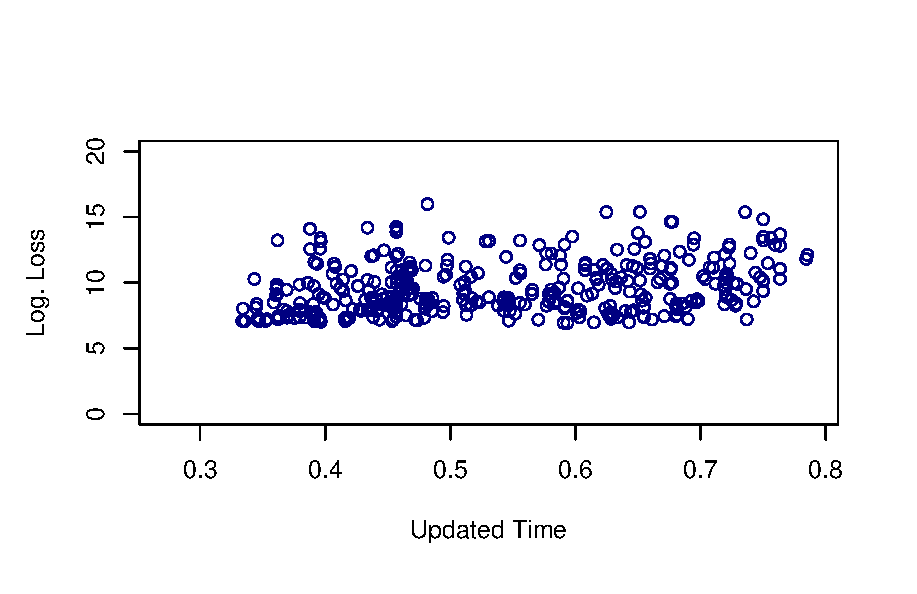
\includegraphics[width=7.5cm]{IntraDayUpdatedTime.eps}
         &
         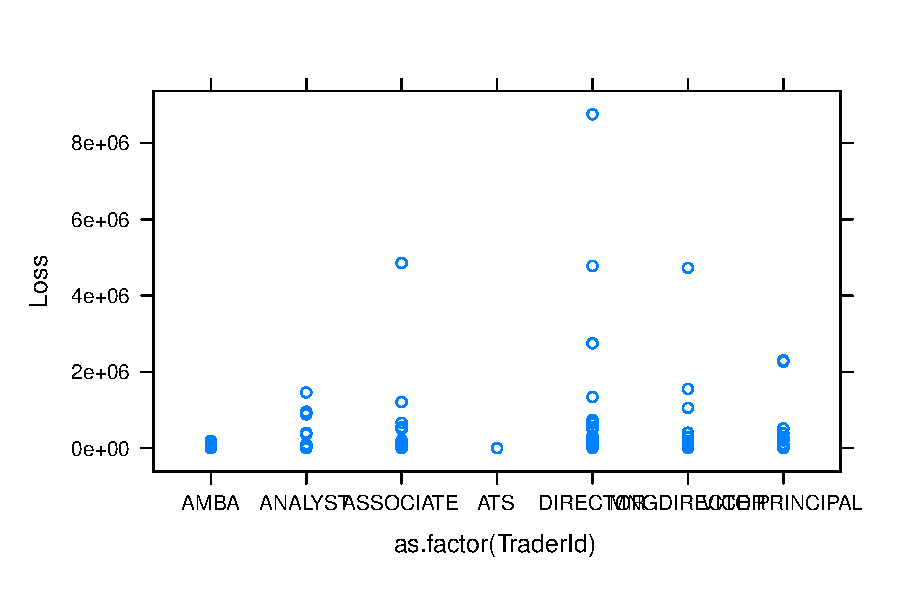
\includegraphics[width=7cm]{TrendTraderId.eps}
         \end{tabular}
    \end{frame}
\subcaption{Scatterplots}
   \label{Intra_Day_Trends} 
\end{subfigure}

\begin{subfigure}[b]{0.55\textwidth}
   \begin{frame}
      \centering
       \begin{tabular}{cc}
        \textbf{Loss per month} & \textbf{Trading frequency} \\
        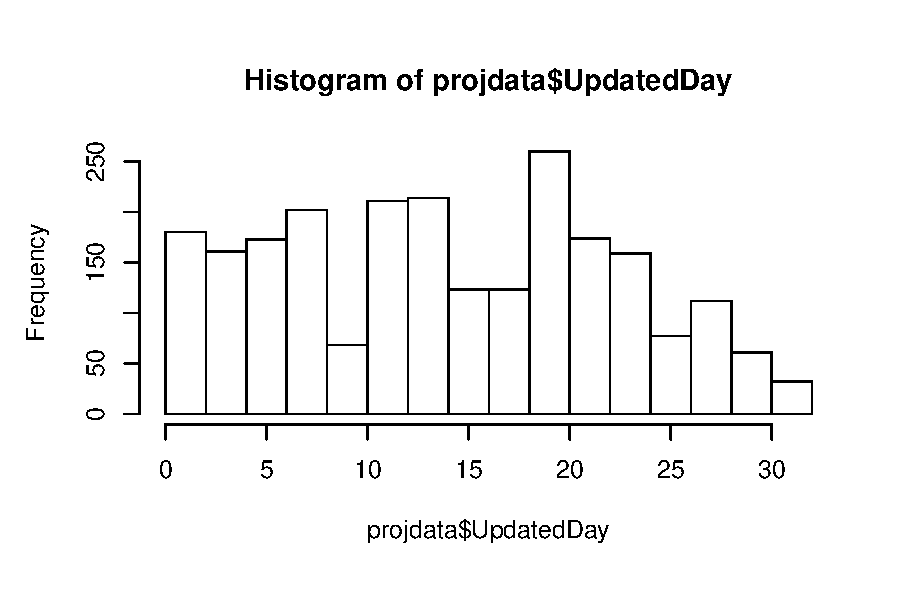
\includegraphics[width=7.5cm]{UpdatedDayFreq.eps}
         &
         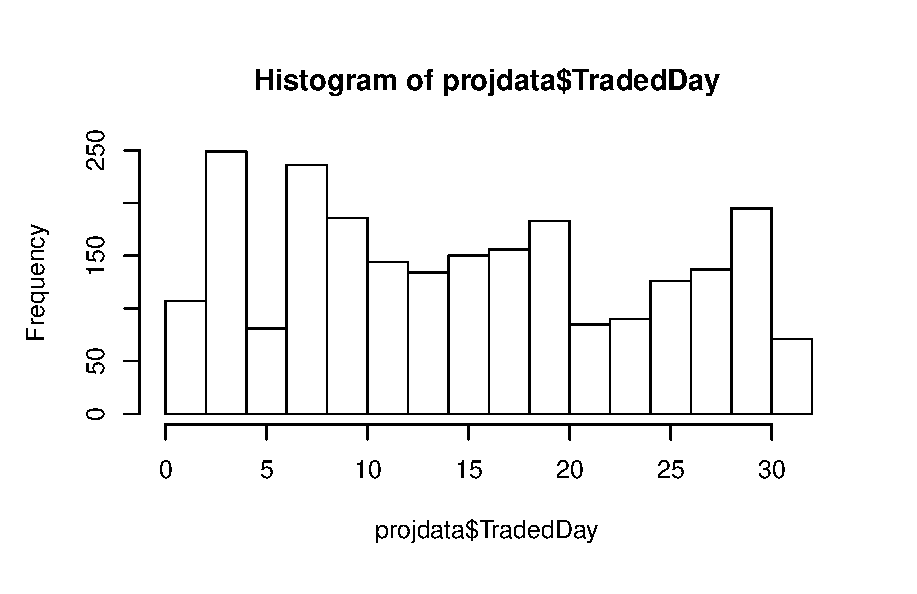
\includegraphics[width=7cm]{TradedDayFreq.eps}
         \end{tabular}
    \end{frame}
\subcaption{Histograms}
   \label{Hist_Loss_Freq}
\end{subfigure}
\caption[Numerical grid display]{(a) Scatterplots of intra-day trend analysis for logs of severities of operational events and trends incident activity for identifying the role of the trader originating the incidents. (b) As for (a) but in the form of histograms showing the frequency distrbution of the number daily operational indicents and the number of trades over a monthly period.} 
\end{figure}

\singlespacing


\end{document}
